\section{Theoretical Analysis}
\label{sec:theoretical}

\par In this section, the circuit shown in figure \ref{fig:1} is analysed theoretically.
\par Like we said in section \ref{sec:introduction}, both of the stages of the amplifier are going to be analysed in a more detailed way in this section.
\par Let's begin with the gain stage. The gain stage consists of a common emitter amplifier, with a NPN transistor, which allows us to obtain a high input impedance ($Z_{i_1}$), and a high gain $A_V$. However, this type of amplifier has a very high output impedance ($Z_{o_1}$), which causes a degeneration of the signal output. In order to solve this problem, the gain stage is connected to an output stage, which consists of a common collector amplifier, whith a PNP transistor. This stage has a gain a little bit lower than 1, but still very close to 1, and a very high input impedance ($Z_{o_2}$), which preserve the high gain of the previous stage. In addition, this circuit has a very low output impedance ($Z_{o_2}$), which means that almost all the gain is going to be delivered to the speaker.

\subsection{First Point}

\par Our theoretical analysis starts by computing the operating point, using the theoretical DC model studied. In order to do this, we harnessed the mesh method provided in the Octave script to which we added the new components.
\par The current directions used are shown in figure \ref{fig:2}, and their values are presented in table \ref{tab:currents}, as well as the values of $V_{CE}$ and $V_{BE}$, and $V_{EC}$ and $V_{EB}$, respectively for the NPN and the PNP transistors, in order to prove that they're working in the forward active region ($V_{CE} > V_{BEON}$ and $V_{EC} > V_{EBON}$).


\vspace{5mm}
\begin{table}[H]
	\centering
	\begin{tabularx}{0.9\textwidth} {
 	    | >{\raggedright\arraybackslash}X
  	    | >{\raggedleft\arraybackslash}X | }
	\hline
	Low Cut Off & 9.090909e+03 rad/s\\ \hline
High Cut Off & 4.545455e+03 rad/s\\ \hline
Medio & 6.428243e+03 rad/s\\ \hline
Input Impedance & 1.000000e+03 \\ \hline
Output Impedance & 3.333333e+02 \\ \hline
Gain & 3.366667e+01 \\ \hline
Gain & 3.054400e+01 dB \\ \hline

	\end{tabularx}
	\caption{$V_{CE}$, $V_{BE}$, $V_{EC}$, $V_{EB}$, and circulation current values}
	\label{tab:currents}
\end{table}
\vspace{5mm}

\subsection{Second Point}

\par The second point in this analysis consists in computing the gain and input and output impedances separately for each stage.
\par In order to do this kind of analysis we have to consider the incremental model of the circuit.


\par In order to compute the gain of each stage, we used the formulae which were taught in the theoretical classes (which were also given in advance in Octave's script). We can use this simplified formulae, because we are assuming medium/high frequencies. Based on this assumption, we can replace the capacitor with a short circuit.
\par In a similar way, we computed the input and output impedances, using the formulae given in the theoretical classes (which were also given in advance in Octave's script), which are based on the same assumption.
\par To make things a little bit more clear, the input/output impedances are determined by connecting, for example, a voltage source to the stage's input/output and replacing the output/input with a short circuit. By determining the current that flows across the added voltage source, we can determine the input/output impedance by just applying Ohm's law. This values are shown in tables 2 and 3, respectively for the input and the output stages. The overall output impedance and gain are shown in table 4.

\vspace{5mm}
\begin{table}[H]
	\centering
	\begin{tabularx}{0.9\textwidth} {
 	    | >{\raggedright\arraybackslash}X
  	    | >{\raggedleft\arraybackslash}X | }
	\hline
	AV1dB & 3.158539e+01 dB\\ \hline
ZI1 & 2.419648e+03 Omega \\ \hline
ZO1 & 4.652785e+03 Omega \\ \hline

	\end{tabularx}
	\caption{Gain, input and output impedances - gain stage}
	\label{tab:stage1}
\end{table}
\vspace{5mm}

\begin{table}[H]
	\centering
	\begin{tabularx}{0.9\textwidth} {
 	    | >{\raggedright\arraybackslash}X
  	    | >{\raggedleft\arraybackslash}X | }
	\hline
	AV2dB & -9.207782e-02 dB\\ \hline
ZI2 & 7.218471e+04 Omega \\ \hline
ZO2 & 3.313468e+00 Omega \\ \hline

	\end{tabularx}
	\caption{Gain, input and output impedances - output stage}
	\label{tab:stage2}
\end{table}
\vspace{5mm}

\begin{table}[H]
	\centering
	\begin{tabularx}{0.9\textwidth} {
 	    | >{\raggedright\arraybackslash}X
  	    | >{\raggedleft\arraybackslash}X | }
	\hline
	AVdB & 3.120876e+01 dB\\ \hline
ZO & 2.270796e+01 Omega\\ \hline

	\end{tabularx}
	\caption{Overal gain and output impedance}
	\label{tab:overall}
\end{table}
\vspace{5mm}

\par As one might observe, the input impedance of the output stage ($Z_{i_2}$) is substantially greater than the output impedance of the gain stage ($Z_{o_1}$). Hence, because the voltage divider applied at the input of the output stage is given by

\begin{equation}
	v_{i_2}= \frac{Z_{i_2}}{Z_{o_1}+Z_{i_2}} \cdot v_{o_1}
\end{equation}

\noindent if $Z_{o_1}<<Z_{i_2}$, we can say that $v_{i_2} \approx v_{o_1}$. It's worth to mention that the gain of the output stage is approximately 1, so overall there is no significant signal loss when the two stages are put together.

\begin{equation}
	AV2dB = -9.207782e-02 \Rightarrow AV2 = 0.989455 \approx 1
\end{equation}

\subsection{Third Point}

\par The third point of this theoretical analysis is to compute the frequency responce $\frac{V_o(f)}{V_i(f)}$. 
\par In order to do so, we can't neglect the effect of the capacitors, since only this component's impedance is frequency dependent.
\par Being that, we calculated the transfer function of the circuit. To do that we calculated the two poles, the lower and high cut off frequency based on the document provided by the professor. Knowing that we built our transfer function and plotted the following figure.

\begin{figure}[H] 
	\centering
	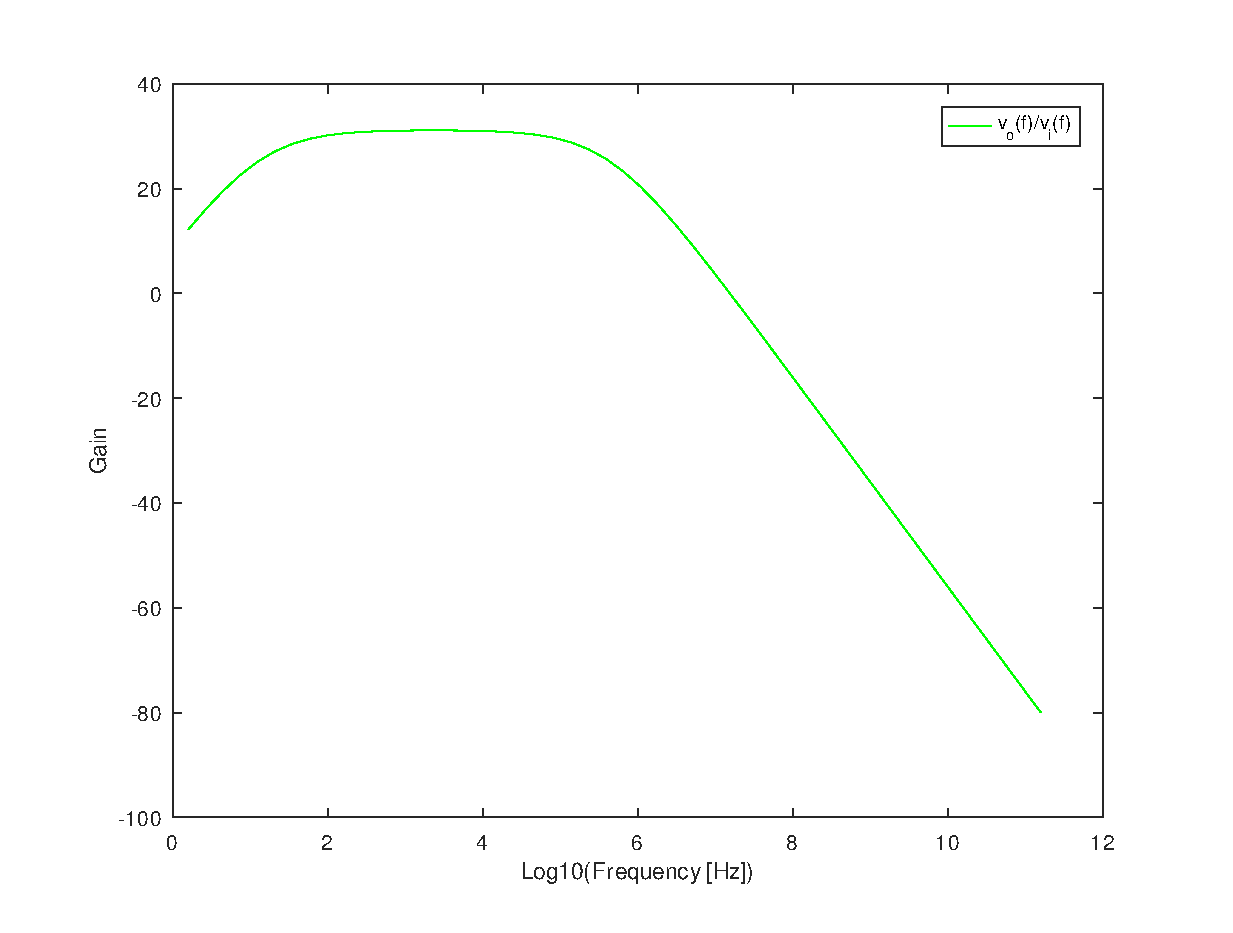
\includegraphics[width=1\linewidth]{teoria.eps}
	\caption{Frequency response of the amplifier ($\frac{V_o(f)}{V_i(f)}$)}
\end{figure}

\par Finally, the theoretical merit is shown below, as well as the high and low cutoff frequencies, the cost and the bandwidth.

\vspace{5mm}
\begin{table}[H]
	\centering
	\begin{tabularx}{0.9\textwidth} {
 	    | >{\raggedright\arraybackslash}X
  	    | >{\raggedleft\arraybackslash}X | }
	\hline
	Merit & 4.921738e+02 \\ \hline
HighCutOff frequency & 4.377991e+05 Hz\\ \hline
LowCutOff frequency & 1.262427e+01 Hz\\ \hline
Cost & 2.198943e+03 MU's\\ \hline
Bandwidth & 4.377865e+05 Hz\\ \hline
Max Gain & 3.111556e+01 V\\ \hline

	\end{tabularx}
	\caption{Theoretical variables of merit}
	\label{tab:merit1}
\end{table}
\vspace{5mm}

